\documentclass{polytech/polytech}

\typereport{stagedi5}

\reportyear{2017-2018}
\title{Réalisation d'un outil de cartographie sur le progiciel Amplitude}
\student{Romain}{ROUSSEAU}{romain.rousseau@etu.univ-tours.fr}
\academicsupervisor{Yannick}{KERGOSIEN}{yannick.kergosien@univ-tours.fr}
\industrialsupervisor[Responsable Cellule Architecture]{Alexandre}{DURAND}{alexandre.durand@soprabanking.com}

\company[images/logoSopra]{Sopra Banking}{47 rue Christiaan Huygens \\ 37073 Tours Cedex 2 - France}{www.soprabanking.com}

\resume{}

\motcle{}

\abstract{}

\keyword{}


%%%%%%%%%%%%%%%%%%%%%%%%%%%%%%%%%%%%%%%%%%%%%%%%%%%%%%%%%%%%%%%%%%%%%%%%%%%%%%%%%%%%%%%%%%%%%%%%%%%
%%%%%%%%%%%%%%%%%%%%%%%%%%%%%%%%%%%%%%%%%%%%%%%%%%%%%%%%%%%%%%%%%%%%%%%%%%%%%%%%%%%%%%%%%%%%%%%%%%%

\begin{document}

\chapter*{Introduction}


Ce rapport présente mon stage d'assistant ingénieur réalisé dans l'entreprise \textit{Sopra Banking Software} à Tours. Le sujet du stage était la réalisation d'un outil de cartographie pour le progiciel nommé \textit{Amplitude} de l'entreprise. Le stage a débuté le 9 avril 2018 avant de s'achever le 31 août de la même année.

Le stage de cinquième année a pour but d'appliquer les connaissances acquises lors des précédentes années d'étude. Il doit représenter une synthèse de l'ensemble des caractéristiques qu'un ingénieur doit avoir dans un environnement concret. Alors que le stage de troisième année sert à découvrir le monde de l'entreprise et que celui de quatrième année sert à faire le premier pas vers le métier d'ingénieur, le stage de dernière année permet de travailler dans une équipe installée pour mener à bien un projet, dans son intégralité ou tout du moins sa majorité selon les cas. Ce stage est censé donner une autonomie supérieure aux étudiants, qui doivent prendre des décisions et avoir la possibilité de donner leur avis sur les opérations en cours, ce qui en fait ainsi, une expérience nécessaire pour le métier. 

Il se déroule sur une période d'au minimum 18 semaines, ce qui permet de pouvoir réaliser des projets avec une envergure dont les étudiants-ingénieurs n'ont jamais eu l'occasion de faire durant leur cursus. Il s'agit du stage le plus important de la formation car il s'agit du plus complet, du plus formateur et de manière générale, du plus intéressant. Il apporte une expérience non négligeable et représente la dernière marche avec l'arrivée dans la vie active.

Le secteur de l'informatique est très porteur et les offres de stage sont donc très nombreuses et variées. L'opportunité de stage dans l'entreprise \textit{Sopra Banking Software} est venue lors du Forum des Entreprises qui se déroule à Polytech pendant le mois de novembre. J'y ai pu rencontrer de nombreux acteurs du secteur et obtenir des entretiens avec plusieurs d'entre eux, dont notamment deux à Sopra sur le site de Tours. À la suite de ces entretiens, j'ai pu faire mon choix parmi les propositions. J'ai retenu celle de la Cellule Architecture de \textit{Sopra Banking Software} pour plusieurs raisons. Tout d'abord, le domaine de la banque m'a toujours intéressé, j'ai déjà fait mon stage de 4ème année chez Worldline du côté des paiements en ligne et je voulais découvrir un autre aspect du domaine. Ensuite, j'avais envie de faire partie d'un projet que ne soit pas monotone et qui me permette d'acquérir de nouvelles connaissances sur des technologies que je ne maîtrise pas ou très peu. Et c'était le cas avec cette offre qui combinait tous les aspects d'un projet, de l'expression des besoins jusqu'au développement en passant par la modélisation ou encore le chiffrage, le tout en utilisant des technologies récentes, variées et performantes. 

Les chapitres qui vont suivre exposeront les principales phases de mon stage, en commençant d'abord par une présentation de l'entreprise et du projet en lui-même. La suite sera consacrée à mon parcours au sein de l'équipe, avec dans un premier temps, une phase de formations sur les différents éléments de l'entreprise ainsi que sur les technologies qui seront utilisées; puis, à la modélisation de l'outil, avec l'élaboration des diagrammes de Gantt, et le chiffrage du projet; et enfin le développement en lui-même. 


\part{Présentation de l'entreprise et du projet}


Cette partie sera consacrée à la présentation du cadre général de mon stage, c'est-à-dire le groupe \textit{Sopra}, sa filiale \textit{Sopra Banking Software}, le progiciel Amplitude et la présentation générale du sujet. 


\chapter{Le groupe \textit{Sopra Steria} et \textit{Sopra Banking Software}}

\section{Histoire des deux groupes: \textit{Sopra} et \textit{Steria}}

\begin{figure}
	
\includegraphics[scale=1]{images/sopralogo}
\end{figure}

\textit{Sopra Steria} est une entreprise de services du numérique qui propose des prestations de conseils, des services technologiques et qui édite des logiciels métiers dans trois principaux domaines: les ressources humaines, l'immobilier et la banque. Définie comme leader européen de la transformation numérique, l'entreprise, de par sa diversité, propose l'un des portefeuilles d'offres les plus complets du marché. L'une des principales motivations du groupe est d'accompagner ses clients dans leur transformation numérique et les aider à faire le meilleur usage de leurs outils. Parmi les actuels clients de l'entreprise, on peut citer des grands noms comme Airbus, La Banque Postale, le Ministère de la Défense, EDF, le Ministère des Finances, la SNCF, Easyjet, et bien d'autres.  

Comme beaucoup de SSII à grandes envergures, \textit{Sopra Steria} est le fruit de nombreuses acquisitions et fusions au fil du temps. Tout d'abord, \textit{Sopra} et \textit{Steria} composaient deux entreprises distinctes. Elles ont toutes les deux été créées à la fin des années 70 (en 1968 pour \textit{Sopra} et en \textit{1968} pour \textit{Steria}). Les deux entreprises se développent dans les années qui suivent. \textit{Sopra} (acronyme pour \textbf{SO}ciété de \textbf{PR}ogrammation et d'\textbf{A}nalyses) investit dans le développement de logiciels, notamment dans le domaine bancaire et les ressources humaines. Le groupe \textit{Sopra} fera son entrée à la bourse de Paris en 1990 après avoir travaillé sur un projet avec Ministère de l'Intérieur. De son côté, \textit{Steria} (acronyme de Société d'étude et de réalisation en informatique et automatisme) réalise de grandes signatures du côté de la sphère publique, en informatisant l'AFP en 1975 ou encore en participant au développement du Minitel en 1981 par exemple. 

Le milieu des années 90 marque le début d'une série d'acquisitions de la part des deux groupes. \textit{Sopra} s'implante au Royaume-Uni, en Espagne, en Italie et en Allemagne en 1999 tandis que \textit{Steria} rentre à la bourse de Paris cette même année. Par la suite, le groupe double de taille en intégrant les activités européennes de \textit{Bull} en 2001 et se renforce dans le conseil en acquérant l'entreprise allemande \textit{Mummert Consulting} en 2005. \textit{Steria} développera considérablement ses parts de marché dans le secteur public au Royaume-Uni en acquérant la société \textit{Xansa}, expert dans le \textit{Business Output Processing}. Le groupe \textit{Sopra} quant à lui, consolide son expansion européen en créant la filiale \textit{Axway Software} en 2001 qui deviendra indépendante en 2011. En parallèle, \textit{Sopra} acquiert 100\% du groupe \textit{Delta Informatique}, société indépendante éditrice d'une offre de solutions « Global Banking » destinée aux banques de détail en France et à l’international. Suite à ce rachat et à celui d'autres sociétés et filiales, en 2012, le groupe \textit{Sopra}, reconnu pour son expertise dans les services financiers, crée la filiale \textit{Sopra Banking Software}. Les solutions dédiées aux ressources humaines feront parties d'une autre filiale appelée, \textit{Sopra HR Software}.

\section{Fusion des deux groupes et création de \textit{Sopra Steria}}


L'année 2014 marquera le rapprochement amical des deux entités. L'OPE du groupe \textit{Sopra} visant la totalité des actions de \textit{Steria} sera un succès. \textit{Sopra Group} devient ainsi \textit{Sopra Steria Group}. Le changement sera effectif le 31 décembre 2014. Suite au plan d'intégration construit conjointement par les équipes des deux entités précédentes, le groupe continue de mener sa politique basée l'acquisition de nouvelles entreprises comme \textit{Cassiopae}, éditeur spécialisé dans les solutions de crédits à l'entreprise et la gestion immobilière locative, \textit{Kentor}, société scandinave spécialisée dans le conseil, l'intégration de systèmes et la maintenance applicative, ou encore \textit{Galitt}, éditeur de solutions sur le marché des systèmes de paiement et des transactions sécurisées.

Le développement continuel du groupe lui permet d'atteindre une place importante parmi les entreprises de services numériques mondiales. Aujourd'hui, le groupe compte plus de 42 000 collaborateurs dans plus de 20 pays à travers le monde et un chiffre d'affaires de 3,8 milliards d'euros en 2017.

\section{La filiale \textit{Sopra Banking Software}}

\begin{figure}
	
\includegraphics[scale=1]{images/logoSopra}
\end{figure}

La filiale \textit{Sopra Banking Software} est un fournisseur de solutions globales comprenant, outre sa gamme de progiciels, les services d'intégration, de support et de conseil associés. Elle a été initiée suite au rachat de plusieurs entreprises du secteur bancaire dont notamment \textit{Delta Informatique} en 2011. Par ailleurs, le site \textit{Sopra Banking Software} de Tours où j'ai réalisé mon stage était auparavant un site \textit{Delta Informatique}.

Ses solutions accompagnent près de 800 banques dans 70 pays. Son objectif est d'accompagner les établissements dans leur développement et dans leur stratégie internationale, par une approche de partenariat à long terme. La société s'appuie pour cela sur l'engagement et l'expertise de plus de 3 500 personnes. Les principales zones d'activités de \textit{Sopra Banking} sont en Europe, en Afrique et au Moyen-Orient. La filiale compte un panel d'offres variées pour les clients. Parmi ces offres, on trouve notamment le progiciel \textit{Amplitude} sur lequel mon stage va se baser. 


\chapter{Le progiciel Amplitude}

\section{Présentation}

\textit{Amplitude}, de son nom complet \textit{Sopra Banking Amplitude}, est la solution de \textit{core banking} proposé par \textit{Sopra Banking Software} pour traiter de manière intégrée toutes les problématiques bancaires. Le progiciel a été développé au sein du groupe \textit{Delta Informatique} avant son acquisition par \textit{Sopra}. \textit{Amplitude} est adoptée par 200 banques dans 50 pays et s’adresse à tous types d’institutions financières, de la banque en création aux grands groupes.

Parmi les avantages listées sur le site de \textit{Sopra Banking}, on retrouve: 

\begin{itemize}
	\item Une large couverture avec plus de 80 modules métiers
	\item Un système entièrement digital ready et sécurisé
	\item Une solution évolutive et agile
	\item Une architecture orientée client et process	
\end{itemize}


\section{Architecture générale}


Branche d'Amplitude


Arborescence


\chapter{Présentation du projet}

Cartographie / Expression des besoins


\part{Tutoriels et formations}


Cette partie sera consacrée aux différents tutoriels et formations que j'ai effectué lors des premières semaines de stage (approximativement les 3 semaines du mois d'Avril). Après avoir pris connaissance du sujet et des locaux, une phase de mise à niveau sur les outils que nous allions utiliser s'imposait. Le principe était de réaliser des tutoriels préconisés par mon encadrant (tutoriels internes à \textit{Sopra} ou sur Internet) et de réaliser des comptes-rendus (ou \textit{Proof of Concept}) sur les outils observés pour que les personnes souhaitant s'intéresser au sujet puissent avoir un support disponible. Les formations étaient portées sur trois technologies principales : \textit{Spring Boot}, \textit{Spring Data} et \textit{Angular}. Ces technologies seront détaillées dans cette partie.


\chapter{Spring Boot}

\textit{Spring Boot} a pour but de faciliter la création d'application utilisant \textit{Spring} en automatisant ses configurations. \textit{Spring Boot} permet par ailleurs de créer pour un projet, un exécutable unique contenant toutes les dépendances nécessaires. Les objectifs annoncés par la documentation de \textit{Spring Boot} sont les suivants : 

\begin{itemize}
	\item Proposer des solutions rapides et accessibles pour les développements \textit{Spring} ;
	\item Faciliter les configurations, même lorsque les paramètres souhaités diffèrent de ceux utilisés par défaut ;
	\item Proposer une panoplie d'options non-fonctionnelles (comme des serveurs embarqués \textit{Tomcat}, des options de sécurité, de mesures de performances, etc.) ;
	\item Aucune génération de code ni de configuration XML. 
\end{itemize}

\textit{Spring Boot} ne génère pas de code ni ne modifie les fichiers du projet. Au démarrage de l'application, \textit{Spring Boot} va dynamiquement « brancher » les composants et les configurations nécessaires au contexte du projet. Les deux principales modifications à opérer pour faire fonctionner \textit{Spring Boot} se passent sur le fichier \textit{Maven} et au travers d’annotations du framework \textit{Spring} sur les composants en action. Le détail du fonctionnement sera détaillé dans les prochaines sections. 

\textit{Spring Boot} fonctionne avec les versions Java 1.8 et supérieur. Les différentes versions des composants utilisés par \textit{Spring Boot} sont détaillés dans le guide de référence à l’adresse suivante : \url{https://docs.spring.io/spring-boot/docs/2.0.1.RELEASE/reference/htmlsingle/}.


\section{Création d'un projet avec \textit{Spring Initializr}}

Il est possible de générer un projet \textit{Spring Boot} avec toutes les dépendances que l’on souhaite \textit{Spring Initializr} à l’adresse : \url{https://start.spring.io/}. Un aperçu du site est visible sur la \autoref{fig:initializr}.

\begin{figure}
	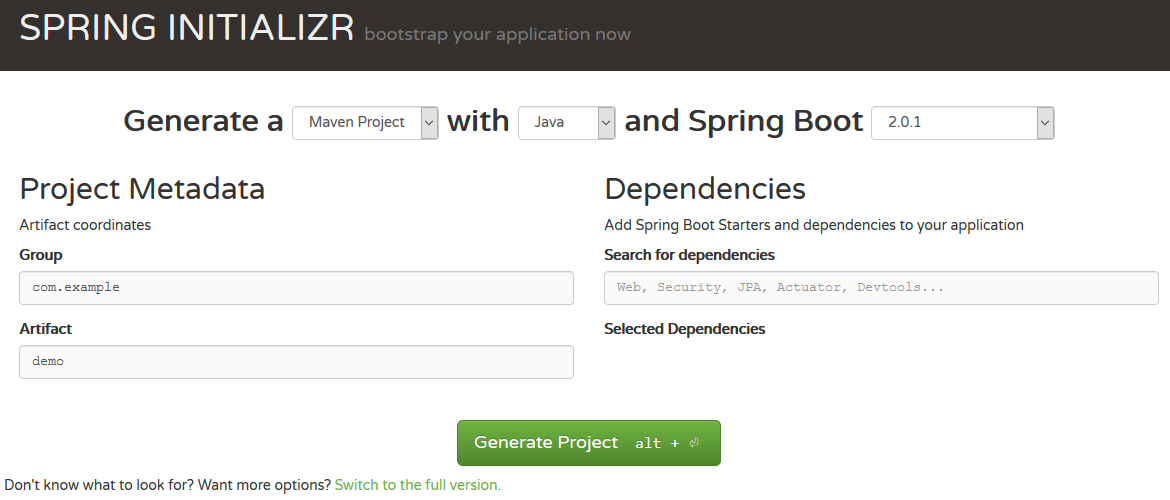
\includegraphics[scale=0.5]{images/springInitializr}
	\caption{Aperçu du site \textit{Spring Initializr}}
	\label{fig:initializr}
\end{figure}

Il suffit d’indiquer les propriétés du projet et les dépendances que l’on souhait ajouter et un modèle de projet \textit{Spring Boot} sera disponible au téléchargement. Les détails et le fonctionnement du fichier \textit{pom.xml} généré sont détaillés dans la prochaine section. 

La création d'un projet par ce biais n'est pas obligatoire, cependant dans les cas où l'on connaît par avance les principales dépendances de notre projet, cela s'avère être un gain de temps non négligeable. Le projet généré est sous forme de dossier compressé \textit{.zip} contenant la structure du projet, le fichier de construction du projet \textit{pom.xml} de \textit{Maven} avec toutes les dépendances, et les classes principales. 


\section{Utilisation avec \textit{Maven}}

\section{title}

\chapter{Spring Data}


\chapter{Angular}


\part{Modélisation de l'outil et chiffrage du projet}


\chapter{Modélisation UML}


\part{Développement}


\chapter{title}


\chapter{Bilan du stage}


\appendix

\end{document}
